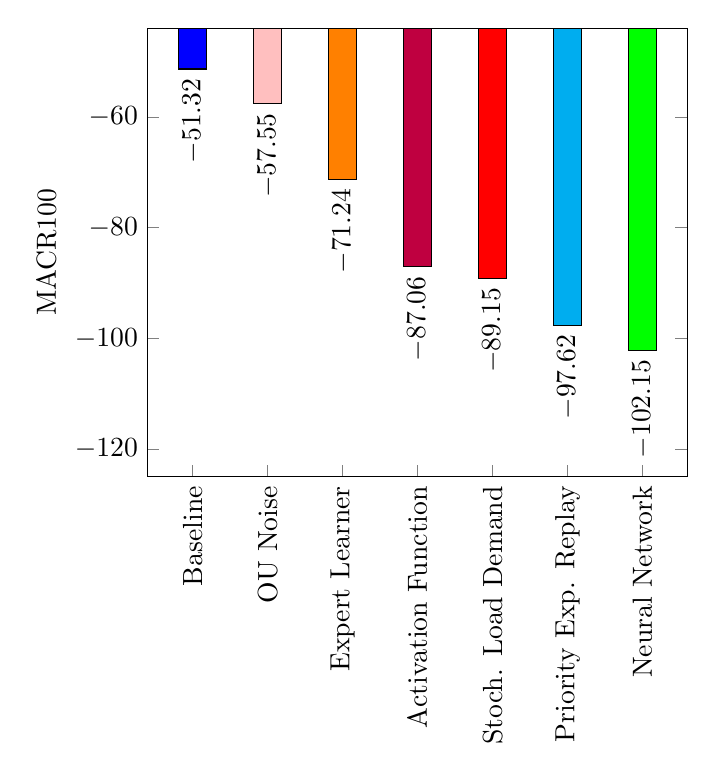
\begin{tikzpicture}
	\begin{axis}[
	    ylabel={MACR100},
	    symbolic x coords={Baseline,, OU Noise,, Expert Learner,, Activation Function,, Stoch. Load Demand,, Priority Exp. Replay,, Neural Network},
	    xtick = {Baseline, Neural Network, Activation Function, OU Noise, Priority Exp. Replay, Expert Learner, Stoch. Load Demand},
	    xticklabel style={rotate=90},
	    nodes near coords,
	    nodes near coords align={vertical},
	    every node near coord/.append style={rotate=90, anchor=east},
	    ymin=-125
	    ]
	\addplot [ybar, fill=blue] coordinates {(Baseline, -51.32)};
	\addplot [ybar, fill=green] coordinates {(Neural Network, -102.15)};
	\addplot [ybar, fill=purple] coordinates {(Activation Function, -87.06)};
	\addplot [ybar, fill=pink] coordinates {(OU Noise, -57.55)};
	\addplot [ybar, fill=cyan] coordinates {(Priority Exp. Replay, -97.62)};
	\addplot [ybar, fill=orange] coordinates {(Expert Learner, -71.24)};
	\addplot [ybar, fill=red] coordinates {(Stoch. Load Demand, -89.15)};
	%\legend{Baseline, Neural Network, Activation Function, OU Noise, Priority Experience Replay, Expert Learner, Stochastic Load Demand};
	\end{axis}
\end{tikzpicture}